\section{Documentos y Código}
\subsection{Documentación}
\begin{compactitem}
  \item \href{https://github.com/dexaxi/TFG_Unity_Package/blob/main/Assets/DUJAL/Documentation/DUJAL%20Documentation.pdf}{Documentación}
  \item \href{https://github.com/dexaxi/TFG_Unity_Package/blob/main/Assets/DUJAL/Documentation/Memoria%20TFG%20%C3%81ngel%20Baeza%20S%C3%A1nchez.pdf}{Memoria}
  \item \href{https://docs.google.com/forms/d/e/1FAIpQLSd1cEq_ghDKNGu-EFjOm2AS5huoM882GzUzjwZkY_DLQak9Fw/viewform?usp=sharing&ouid=100594158238727737282}{Cuestionario}
\end{compactitem}

\subsection{Repositorios}
\begin{compactitem}
  \item DUJAL: \url{https://github.com/dexaxi/TFG_unity_package}
  \item UniTask: \url{https://github.com/Cysharp/UniTask}
\end{compactitem}


\section{Tablas y figuras}
\subsection{Resultados del Cuestionario}
% Insertar una figura
\begin{figure}[H]
  \centering
  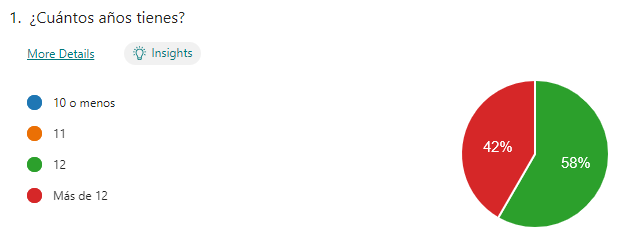
\includegraphics[width=450px,clip=true]{questionario_1.png}
  \caption{¿Cuántos años tienes?}
  \label{fig:questionario_1}
\end{figure}
\raggedbottom


% También con \pagebreak